\documentclass[11pt]{article}
    \usepackage{caption}
    \usepackage{graphicx}
    \usepackage{mathtools}
    \graphicspath{ {img/} }
    \setlength{\parindent}{0pt}
    \DeclareCaptionType{equ}[][]
    \usepackage[svgnames]{xcolor}
    \newcommand\tab[1][1cm]{\hspace*{#1}}    
    \newcommand*{\plogo}{\fbox{$\mathcal{BM}$}}
        
    \usepackage{PTSerif}
     
    \begin{document} 
        
    \begin{titlepage}
    
        \raggedleft
        
        \vspace*{\baselineskip}
        
        {\Large Bryan Melanson}
        
        \vspace*{0.167\textheight}
        
        \textbf{\LARGE How to Not Fail}\\[\baselineskip]
        
        {\textcolor{Red}{\Huge Control Systems}}\\[\baselineskip]
        
        {\Large \textit{While never going to class}}
        
        \vfill
        
        {\large Computer Engineering 2020 ~~\plogo}
        
        \vspace*{3\baselineskip}
    
    \end{titlepage}

    \pagebreak

    %%%%%%%%%%%%%%%%%%%%%%%%%%%%%%%%%%%%%%%%%%%%%%%%%%%

    \tableofcontents

    \pagebreak

    %%%%%%%%%%%%%%%%%%%%%%%%%%%%%%%%%%%%%%%%%%%%%%%%%%%


    \section{Introduction}

    \subsection{System Configuration}

    \begin{center}
        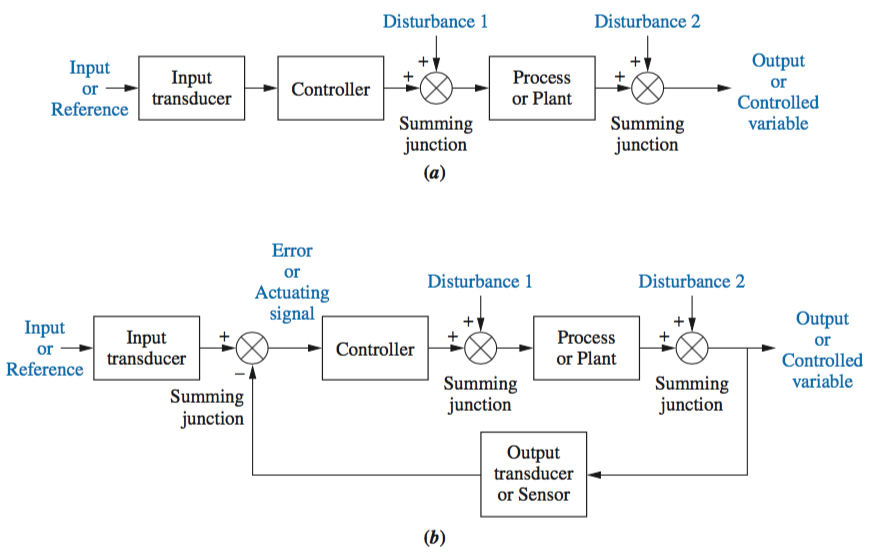
\includegraphics[width=300 px]{img/system-blocks}
    \end{center}

    \textbf{Open Loop} systems do not monitor or correct the output for disturbances; however, they are simpler and less expensive than closed-loop systems. \\ 

    \textbf{Closed Loop} systems monitor the output and compare it to the input. If an error is detected, the system corrects the output and hence corrects the effects of disturbances.

    \subsection{Analysis and Design Objectives}

    \subsubsection{Transient Response}

    That part of the response curve due to the system and the way the system acquires or dissipates energy. In stable systems it is the part of the response plot prior to the steady-state response.

    \subsubsection{Steady-State Response}

    Also known as \textbf{Forced Response}, for linear systems, that part of the total response function due to the input. It is typically of the same form as the input and its derivatives.

    \subsubsection{Stability}

    That characteristic of a system defined by a natural response that decays to zero as time approaches infinity.

    \pagebreak

    %%%%%%%%%%%%%%%%%%%%%%%%%%%%%%%%%%%%%%%%%%%%%%%%%%%

    \section{Modeling in the Frequency Domain}

    \pagebreak

    %%%%%%%%%%%%%%%%%%%%%%%%%%%%%%%%%%%%%%%%%%%%%%%%%%%
    
    \section{Time Response}
    
    \pagebreak

    %%%%%%%%%%%%%%%%%%%%%%%%%%%%%%%%%%%%%%%%%%%%%%%%%%%
    
    \section{Reduction of Multiple Systems}

    \subsection{Block Diagrams}

    The block diagram of a linear, time-invariant system consists of four elements: \textit{signals, systems, summing junctions}, and \textit{pickoff points}. These elements can be assembled into three basic forms: \textit{cascade, parallel}, and \textit{feedback}.

    \begin{center}
        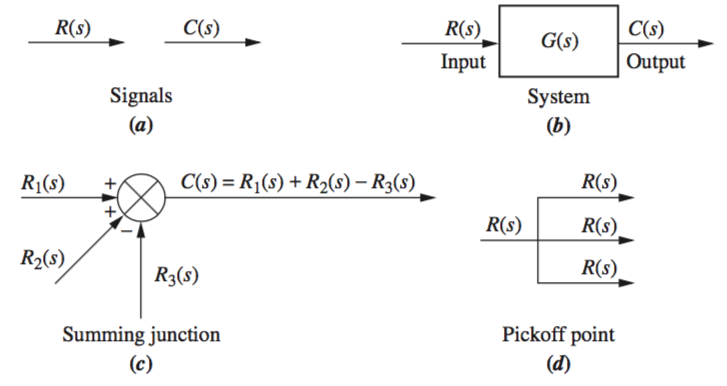
\includegraphics[width=300 px]{img/reduction} \\
    \end{center}

    \subsubsection{Cascade Form}

    \begin{center}
        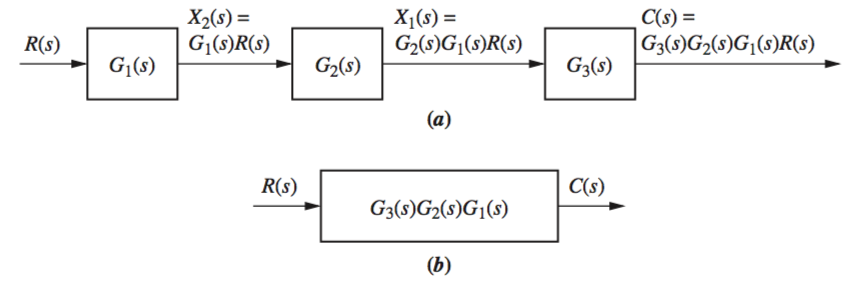
\includegraphics[width=300 px]{img/cascade} \\
    \end{center}

    \subsubsection{Parallel Form}

    \begin{center}
        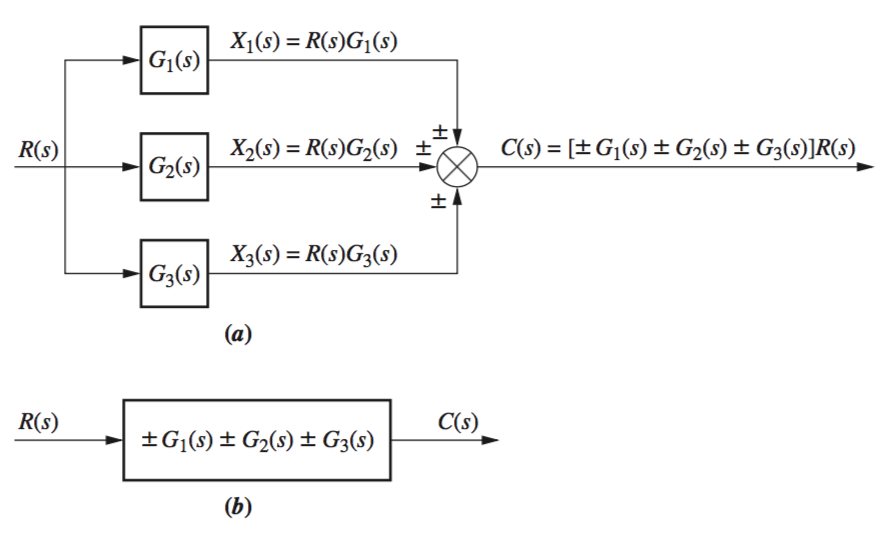
\includegraphics[width=300 px]{img/parallel} \\
    \end{center}

    From the above diagram, it is clear that each branch will be $R(s)G_1(s)$, $R(s)G_2(s)$, or $R(s)G_3(s)$, and when the three are summed at the summer, $R(s)[G_1(s) + G_2(s) + G_3(s)]$. 

    \subsubsection{Feedback Form}

    \begin{center}
        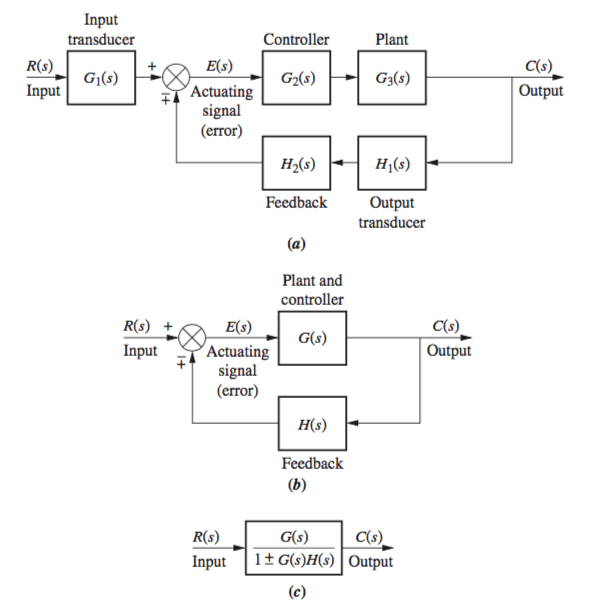
\includegraphics[width=300 px]{img/feedback} \\
    \end{center}

    \subsubsection{Moving Blocks}

    From these diagrams, the logic of moving each process can be validated when summing each signal and multiplying by each process, then doing the same for its equivalent system. \\
    
    $[R(s) + X(s)] * G(s) = R(s)G(s) + X(s)G(s)$  $\equiv$
    $R(s)G(s) + X(s)G(s) = C(s)$

    \begin{center}
        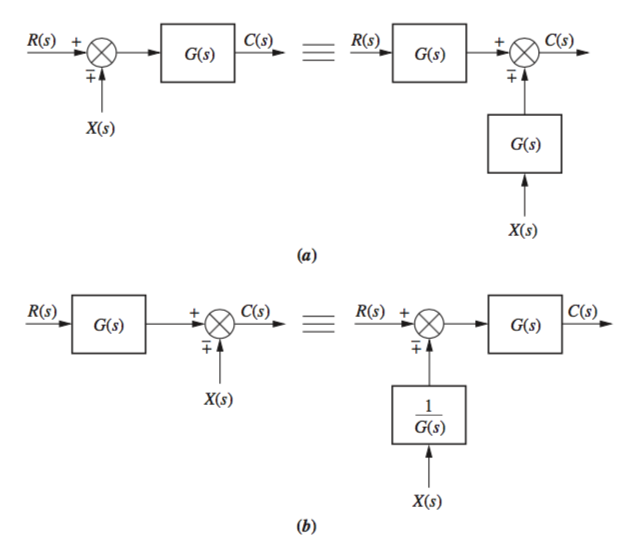
\includegraphics[width=300 px]{img/move1}
        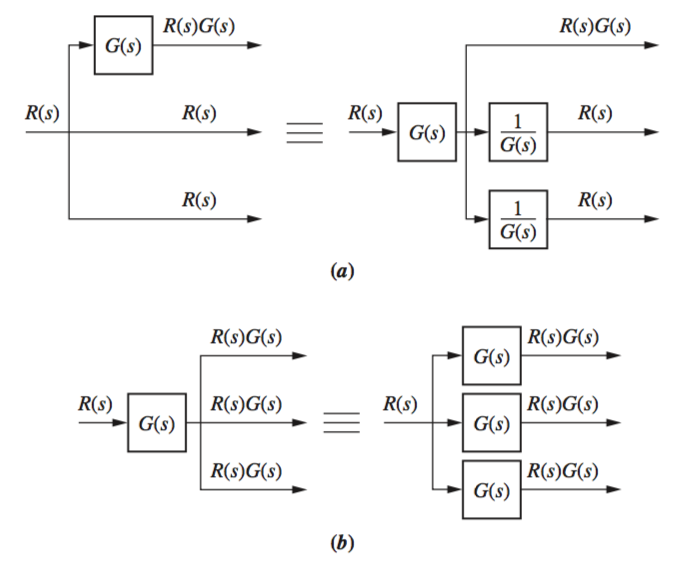
\includegraphics[width=300 px]{img/move2}
    \end{center}
    
    \pagebreak

    %%%%%%%%%%%%%%%%%%%%%%%%%%%%%%%%%%%%%%%%%%%%%%%%%%%

    \section{Stability}
    \subsection{Routh-Hurwitz Criteria}

    \begin{center}
        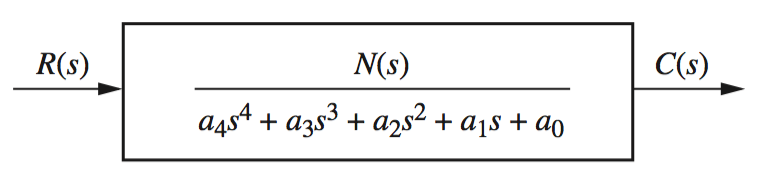
\includegraphics[width=300 px]{img/routh-1}
        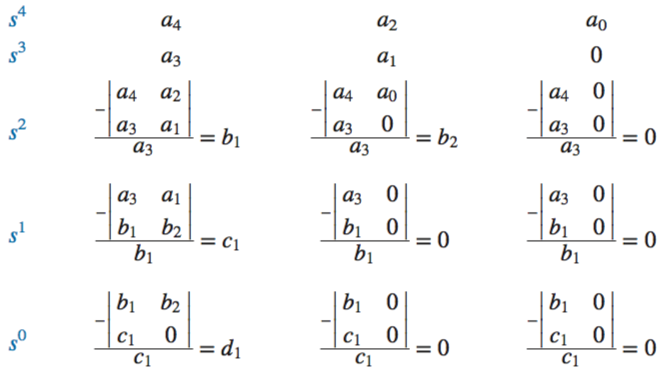
\includegraphics[width=300 px]{img/routh-2}
    \end{center}

    \subsection{Routh-Hurwitz Special Cases}

    \subsubsection{Zero Only in the First Column}

    \begin{center}
        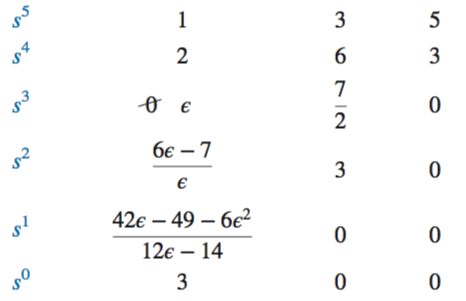
\includegraphics[width=300 px]{img/routh-e}
        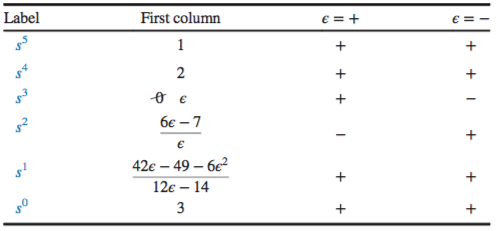
\includegraphics[width=300 px]{img/routh-e2}
    \end{center}

    Assume a value for the variable $\epsilon$, and follow through the system, tracking sign changes. This should be the same for either assumed value of $\epsilon$. \\ 

    Alternately, the reverse coefficients of the denominator can be used in analysis, as seen below:

    \begin{center}
        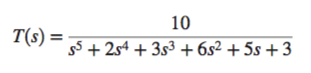
\includegraphics[width=300 px]{img/routh-recip}
        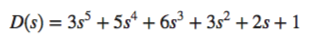
\includegraphics[width=300 px]{img/routh-recip2}
    \end{center}
    
    \subsubsection{Entire Row Is Zero}

    If an entire row is zero, return to the row above, and form the equation represented by those coefficients. For example, from the system below, at row $s^3$ there is a row of zeroes. From the row $s^4$ above, form the equation $s^4 + 6s^2 + 8$. The derivative of this equation will take the place of the row of zeroes. Therefore, $4s^3 + 12s + 0$ will take the place of the zeroes in row $s^3$.

    \begin{center}
        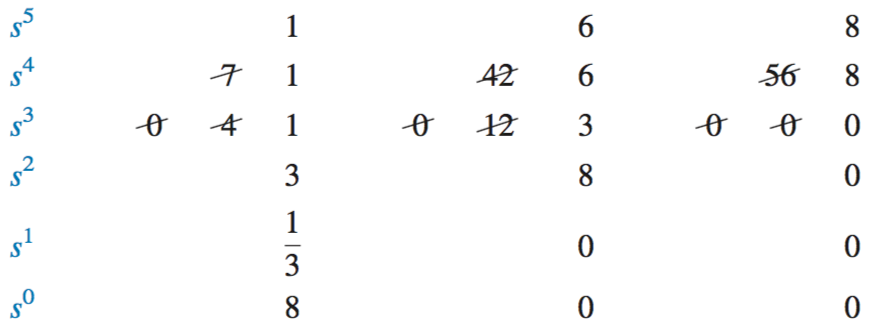
\includegraphics[width=300 px]{img/routh-roz}
    \end{center}

    In the case of a row of zeroes formed by a row of even polynomials, for example $s^4 + s^2 + 1$, it can be determined that its roots are symmetric about the origin. If we don't have a row of zeroes, we cannot have roots on the $jw$-axis. Once a row of zeroes is found for an even polynomial, everything from that row to the end is a test of only the even polynomial. Because in the example above, the zeroes occur in the $s^3$ row, it's considered the $s^4$ row that causes the zeroes, and it is therefore even.

    \begin{center}
        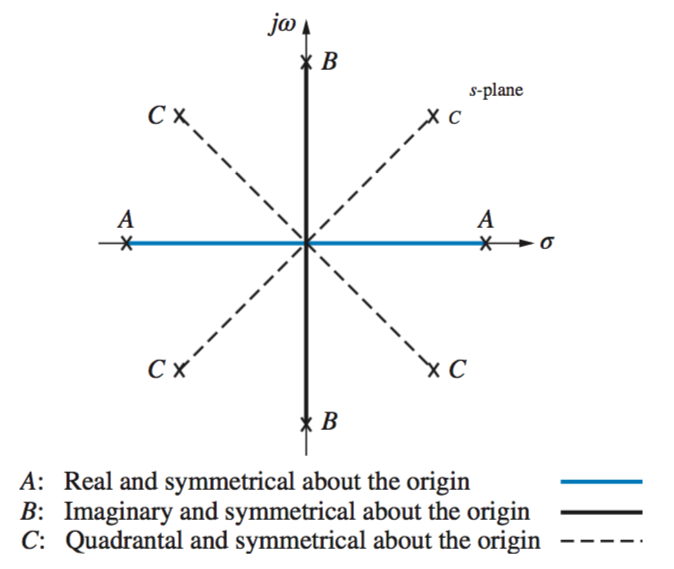
\includegraphics[width=300 px]{img/routh-zeroes}
    \end{center}

    \begin{center}
        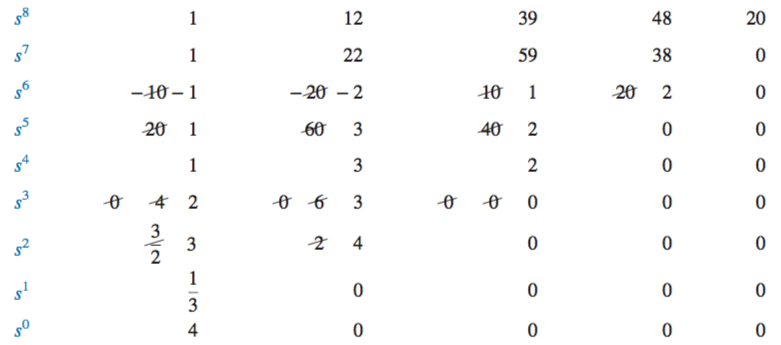
\includegraphics[width=300 px]{img/routh-roz-analysis}
    \end{center}

    From the example above, the row of zeroes can be seen to occur in the $s^4$ row. The rest of rows are therefore a test of the even polynomial, where it is determined there are no changes in sign. Thus, there are no poles in the right half plane, and no left plane poles can exist due to symmetry. Therefore, all four poles must be on the $jw$-axis. \\ 

    The findings for the even polynomials are then combined with the findings for the rest of the system: \\

    \begin{center}
        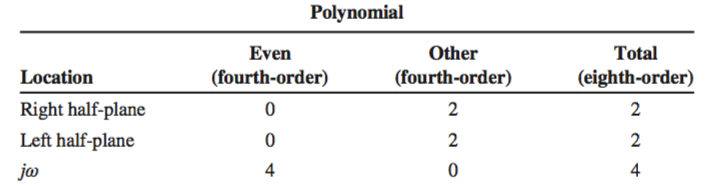
\includegraphics[width=300 px]{img/routh-even}
    \end{center}

    \pagebreak
    
    \pagebreak

    %%%%%%%%%%%%%%%%%%%%%%%%%%%%%%%%%%%%%%%%%%%%%%%%%%%

    \section{Steady State Errors}

    \textit{Steady State Error} is defined as the difference between the input and output as t $\rightarrow \infty$. When testing for factors such as constant position, constant velocity and constant acceleration, inputs such as unit steps $u(t)$, ramps $r(t)$ and parabolas are used. This discussion is limited to stable systems.\\
   
    \begin{center}
        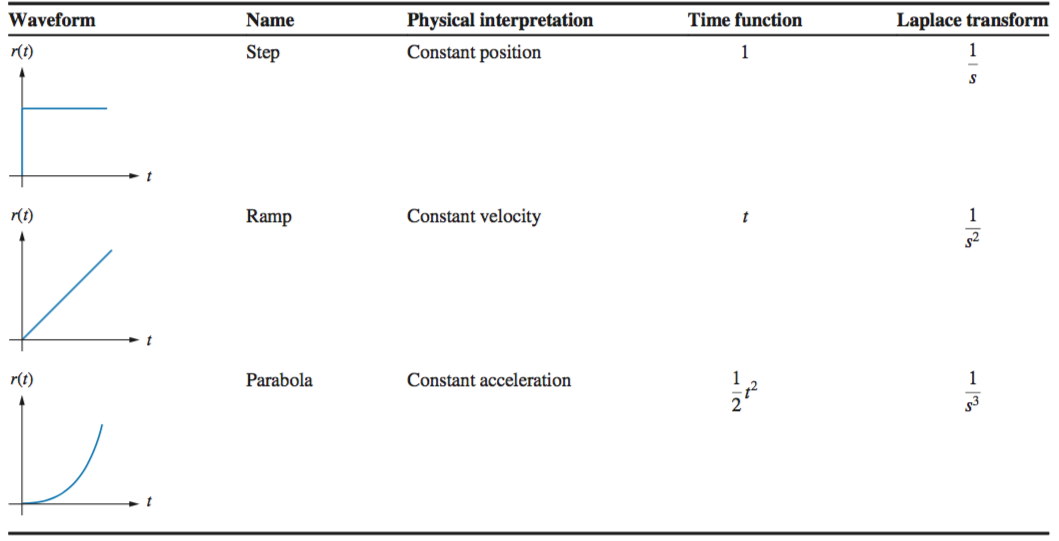
\includegraphics[width=300 px]{img/inputs} \\
    \end{center}

    Most steady state errors $E(s)$ arise from the input and/or the configuration of the system, as seen in the diagrams below for general closed loop and unity feedback systems.

    \begin{center}
        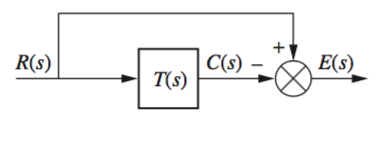
\includegraphics[width=300 px]{img/closedlooperror} \\
    \end{center}

    \begin{center}
        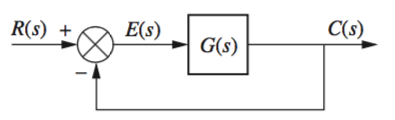
\includegraphics[width=300 px]{img/unityfeedback} \\
    \end{center}
    
    In the first case $E(s) = R(s) - C(s)$ is the error. If the input $R(s)$ is a step input, then $C(s)$ should $= R(s)$ and $E(s) = 0$. However, if gain $K$ is introduced, $C(s) = KR(s)$ and $E(s)$ must be finite and non-zero. \\
    
    \begin{center}
        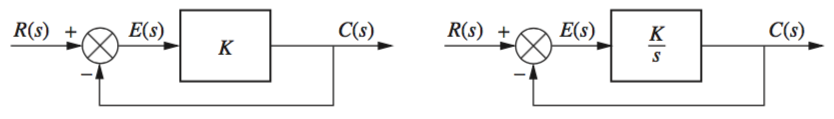
\includegraphics[width=300 px]{img/integrator} \\
    \end{center}

    From these systems we see that $C(s)$ = $KE(s)$, or $E(s) = \frac{1}{K}C(s)$

    \subsection{Steady State Error for Unity Feedback Systems}

    Steady-state error can be calculated from transfer function $T(s)$ or the open loop transfer function $G(s)$. Once $E(s)$ is found, the steady state error can be found using the \textit{Final Value Theorem}, which states that the value at infinity is equal to the Laplace as $s \rightarrow 0$.

    \begin{center}
        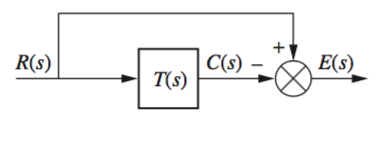
\includegraphics[width=300 px]{img/closedlooperror} \\
    \end{center}

    \begin{center}
        $E(s) = R(s) - C(s)$ \\
        $C(s) = R(s)T(s)$ \\ 
        $E(s) = R(s)[1 - T(s)]$ \\
        $e(\infty) = \text{lim}_{s\rightarrow \infty}  e(t) = \text{lim}_{s\rightarrow 0}  sE(s)$ \\ 
        $e(\infty) = \text{lim}_{s\rightarrow 0} sR(s)[1 - T(s)]$ \\
    \end{center}

    \subsubsection{Steady State Error in Terms of G(s)}

    \begin{center}
        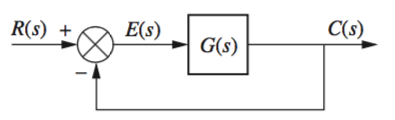
\includegraphics[width=300 px]{img/unityfeedback} \\
    \end{center}

    \begin{center}
        $E(s) = R(s) - C(s)$ \\
        $C(s) = E(s)G(s)$ \\ 
        $E(s) = \frac{R(s)}{1 + G(s)}$ \\
        $e(\infty) = \text{lim}_{s\rightarrow \infty} \frac{sR(s)}{1 + G(s)} $ \\ 
    \end{center}

    \subsection{Static Error Constants and System Type}

    The steady-state error for unit step inputs is \\ 

    $e(\infty) = \frac{1}{1 + \text{lim}_{s\rightarrow 0} G(s)}$ \\
    
    The steady-state error for ramp inputs of unit velocity is \\
    
    $e(\infty) = \frac{1}{\text{lim}_{s\rightarrow 0} sG(s)}$ \\

    The steady-state error for parabolic inputs of unit acceleration is \\
    
    $e(\infty) = \frac{1}{\text{lim}_{s\rightarrow 0} s^2G(s)}$ \\

    The terms in the denominator are known as $k_p, k_v, k_a$, the \textbf{static error constants}, representing position, velocity and acceleration, respectively. \\
    
    Systems can also be defined by \textbf{system type}. This defines the number of pure integrations in the forward path, assuming a unity feedback system. Increasing the system type decreases the steady-state error as long as the system is stable.

    \begin{center}
        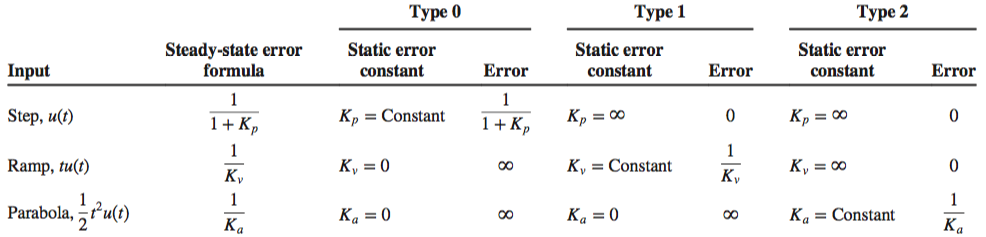
\includegraphics[width=300 px]{img/types} \\
    \end{center}

    This will also be apparent by the structure of the system. An $s$ factor in the denominator which won't cancel with $u(t)$ input indicates the system is not Type 0. Therefore, testing with a ramp and parabola input will determine whether the static constant is finite for each input.

    \subsection{Steady-State Error Specifications}

   The steady-state error is inversely proportional to the static error constant - the larger the constant, the smaller the steady-state erorr. Increasing gain increases the static error constant, thus, increasing the gain decreases the steady-state error if the system is stable.

   \subsection{Steady State Disturbances}

   \begin{center}
    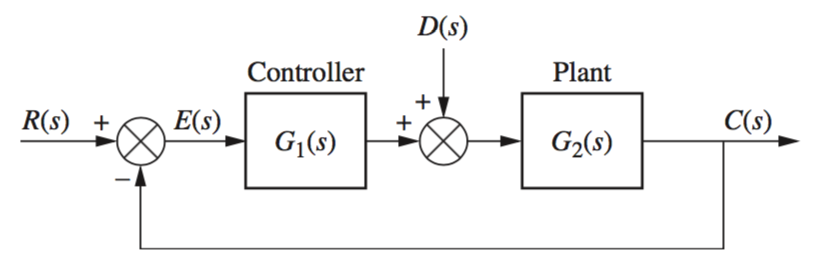
\includegraphics[width=300 px]{img/disturbance} \\
    \end{center}

    $C(s) = E(s)G_1(s)G_2(s) + D(s)G_2(s)$ \\
    
    However, $C(s) = R(s) - E(s)$, therefore, \\
    
    $E(s) = \frac{1}{1 + G_1(s)G_2(s)}R(s) - \frac{G_2(s)}{1+G_1(s)G_2(s)}D(s)$ \\
    
    $e(\infty) = \frac{s}{1 + G_1(s)G_2(s)}R(s) - \frac{sG_2(s)}{1+G_1(s)G_2(s)}D(s)$ \\ 

    $e(\infty) = e_R(\infty) + e_D(\infty)$


   \subsection{Forming Equivalent Unity from Non-Unity Systems}

   \begin{center}
    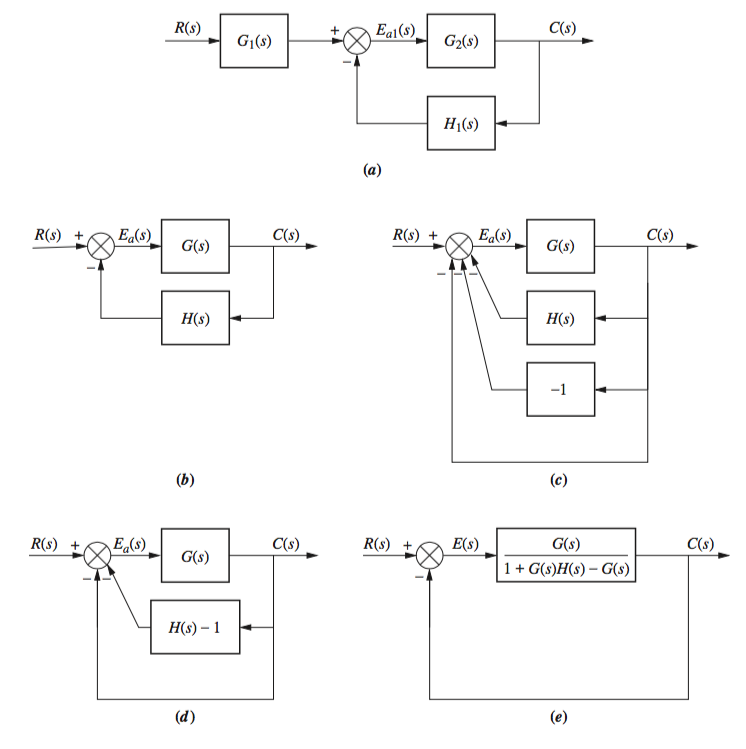
\includegraphics[width=300 px]{img/nonunity} \\
    \end{center}

    \pagebreak

    %%%%%%%%%%%%%%%%%%%%%%%%%%%%%%%%%%%%%%%%%%%%%%%%%%%

    \section{Root Locus Techniques}

    The following sections apply to \textbf{Negative Feedback Closed Loop} systems.

    \subsection{Sketching the Root Locus}

    \subsubsection{Number of Branches}

    The number of branches in a root locus equal the number of poles.

    \subsubsection{Symmetry}

    The root locus is symmetrical about the real axis.

    \subsubsection{Real Axis Segments}

    On the real axis, for $K > 0$ the root locus exists to the left of an odd number of real-axis, finite open-loop poles and/or finite open-loop zeros.

    \subsubsection{Starting and Ending Points}

    The root locus begins at the finite and infinite poles of $G(s)H(s)$ and ends at the finite and infinite zeros of $G(s)H(s)$.

    \subsubsection{Behavior at Infinity}

    \begin{center}
    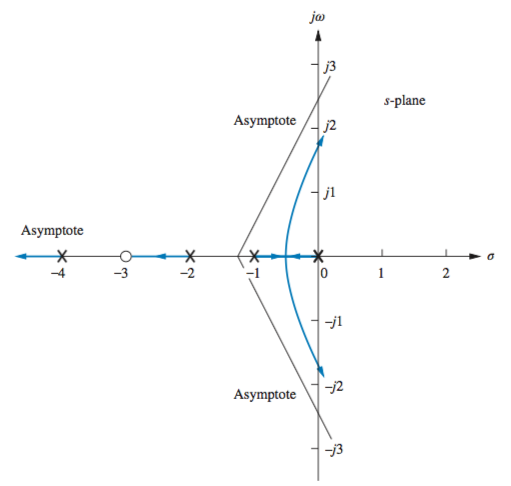
\includegraphics[width=300 px]{img/asymptotes} \\
    \end{center}

    When finding $K$, remember that the denominator of the transfer function $T(s)$, $1 + KG(s)H(s) = 0$ if the point is on the root locus. Set $s$ to a known point on the root locus (break in points work) and solve $1 + KG(s)H(s) = 0$ for $K$.

    \subsection{Refining the Sketch}

    \subsubsection{Breakaway/Break-in Point}

    At the breakaway or break-in point, the branches of the root locus form an angle of 180°/$n$ with the real axis, where $n$ is the number of closed-loop poles arriving at or departing from the single breakaway or break-in point on the real axis. These are the points when gain is at its minimum and maximum, respectively. \\
        
    For all points on the root locus, \\
    
    $K = -\frac{1}{G(s)H(s)}$, $\frac{1}{G(s)H(s)} = -1$ and by differential calculus, \\
    
    $dK = 0$ will $\sigma$, whose zeroes will produce the break-in points.

    \begin{center}
        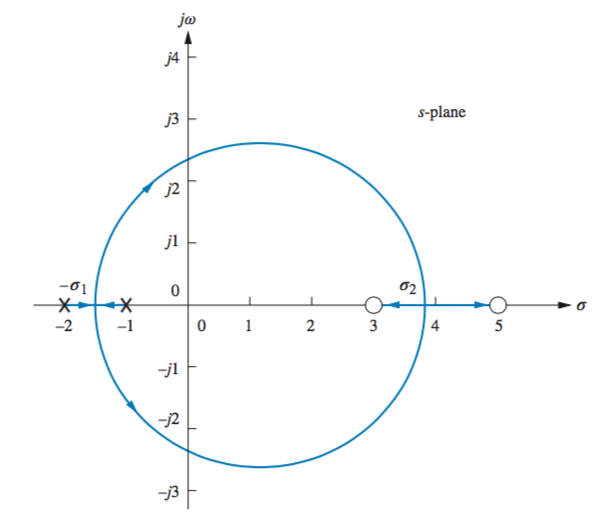
\includegraphics[width=300 px]{img/breakpoints} \\
    \end{center}

    Or, conversely, \\

    $\sum \frac{1}{\sigma + z_i} = \sum \frac{1}{\sigma + p_i}$ \\

    Where $z$ and $p$ are the zero and pole values. By equating the two sides and simplifying to a single equation, factoring can produce $\sigma$.

    \subsubsection{$j\omega$-Axis Crossings}

    The crossing of the $j\omega$ axis defines when the system becomes unstable. The crossing of the $\omega$ axis deines the frequency of oscillation, while the gain at the $j\omega$ axis yields the maximum positive gain for system stability. \\ 

    The $j\omega$ axis crossings can be found using the Routh-Hurwitz criterion. Forcing a row of zeros yields the gain, then going back a row and solving for the roots yields the frequency at the imaginary axis crossing.

    \subsubsection{Angles of Departure and Arrival}

    If we assume a point on the root locus $\epsilon$ close to a complex \textbf{pole}, the sum of angles drawn from all finite poles and zeros to this point is an odd multiple of 180$^\circ$. Except for the \textbf{pole} that is $\epsilon$ close to the point, we assume all angles drawn from all other poles and zeros are drawn directly to the \textbf{pole} that is near the point. Thus, the only unknown angle in the sum is the angle drawn from the \textbf{pole} that is $\epsilon$ close. We can solve for this unknown angle, which is also the angle of departure from this complex \textbf{pole}. \\

    $-\theta_1 + \theta_2 + \theta_3 - \theta_4 - \theta_5 + \theta_6 =…(2k+1)180^\circ$ \\ 
    
    \textit{or} \\ 

    $\theta_1 = \theta_2 + \theta_3 - \theta_4 - \theta_5 + \theta_6 -…(2k+1)180^\circ$ \\

    \begin{center}
        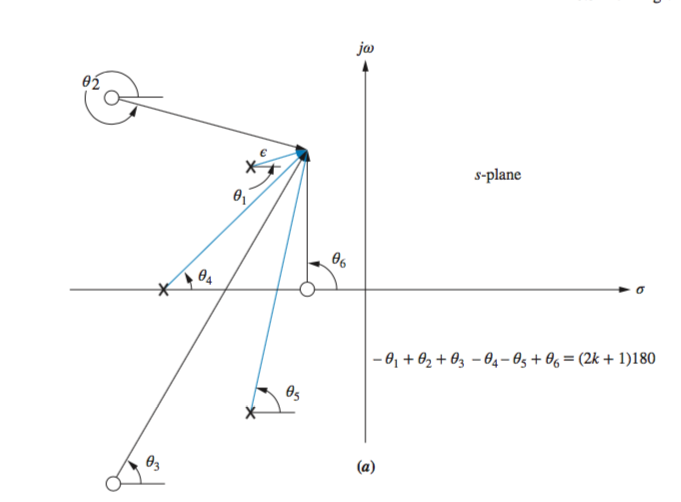
\includegraphics[width=300 px]{img/angles-pole} \\
    \end{center}    
    
    If we assume a point on the root locus $\epsilon$ close to a complex \textbf{zero}, the sum of angles drawn from all finite poles and zeros to this point is an odd multiple of 180$^\circ$. Except for the \textbf{zero} that is $\epsilon$ close to the point, we can assume all angles drawn from all other poles and zeros are drawn directly to the \textbf{zero} that is near the point. Thus, the only unknown angle in the sum is the angle drawn from the \textbf{zero} that is $\epsilon$ close. We can solve for this unknown angle, which is also the angle of arrival to this complex \textbf{zero}. \\ 

    $-\theta_1 + \theta_2 + \theta_3 - \theta_4 - \theta_5 + \theta_6 =…(2k+1)180^\circ$ \\ 
    
    \textit{or} \\ 

    $\theta_2 = \theta_1 - \theta_3 + \theta_4 + \theta_5 - \theta_6 -…(2k+1)180^\circ$ \\

    \begin{center}
        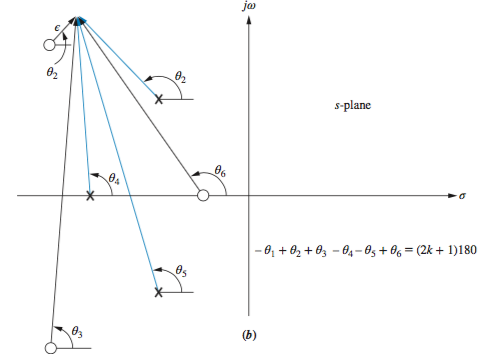
\includegraphics[width=300 px]{img/angles-zero} \\
    \end{center}  

    Note that finding the angle at these points is calculating the length from the poles or zeroes to this point.

    \subsection{Plotting and Calibrating the Root Locus}

    When locating points on the root locus and finding their specified gain, for example as it crosses the radial line representing 20\% overshoot, such as the below graph where $\zeta = 0.45$ \\ 

    Evaluating the graph at points along the line, and summing the angles from poles and zeros, it can be determined if a point is on the root locus if the angles are a multiple of 180$^\circ$.

    \begin{center}
        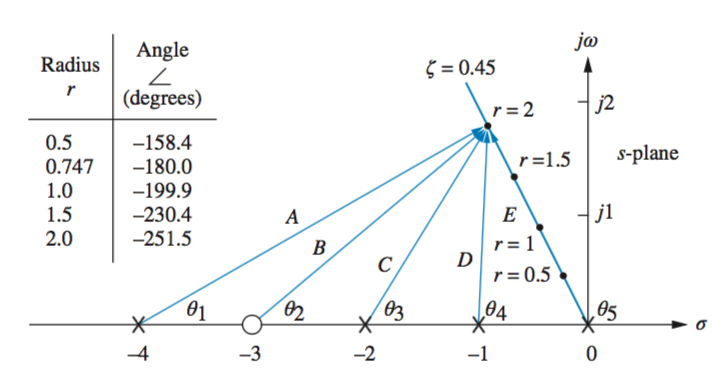
\includegraphics[width=300 px]{img/calibrating} \\
    \end{center}  

    $\zeta = cos(\theta)$, therefore $cos^{-1}\zeta = \theta$ \\ 

    From this value $\theta$, the $x$ and $y$ components of the radial line can be plotted, using cos$\theta$, sin$\theta$, and $r$sin$\theta$, $r$cos$\theta$ to find the components of each radius. 

    \subsection{Generalized Root Locus}

    If finding the root locus of a system concerning a single parameter instead of gain $K$, an equivalent system can be used where the denominator is represented as $1 + p_1G(s)H(s)$. From the below system,\\ 
    \begin{center}
    $T(s) = \frac{KG(s)H(s)}{1 + KG(s)H(s)} = \frac{10}{s^2 + (p_1 +2)s + 2p_1 + 10} = \frac{10}{s^2 + 2s + 10 + p_1(s + 2)}$
    \end{center}

    \begin{center}
        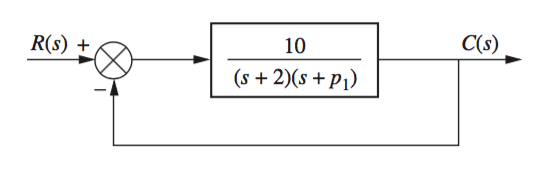
\includegraphics[width=300 px]{img/parameter1} \\
    \end{center}


    \subsection{Positive Feedback Systems}

    $KG(s)H(s) = 1 =ˆ1 \angle k360^\circ \tab k = 0, 1, 2, 3... $

    \begin{enumerate}
        \item \textbf{Number of Branches} \\
        No change
        \item \textbf{Symmetry} \\
        No change
        \item \textbf{Real Axis Segments} \\
        On the real axis, the root locus for positive-feedback systems exists to the left of an \textbf{even} number of real-axis, finite open-loop poles and/or finite open-loop zeros.
        \item \textbf{Starting and Ending Points} \\
        The root locus for positive-feedback systems begins at the finite and infinite poles of $G(s)H(s)$ and ends at the finite and infinite zeros of $G(s)H(s)$.
        \item \textbf{Behavior at Infinity} \\        
        The root locus approaches straight lines as asymptotes as the locus approaches infinity. Further, the equations of the asymptotes for positive-feedback systems are given by the real-axis intercept, $\sigma_a$, and angle, $\theta_a$, as follows: \\
        \begin{center}
            $\sigma_a = \frac{\sum Finite Poles - \sum Finite Zeros}{\# Finite Poles - \# Finite Zeros}$ \\

            $\theta_a = \frac{k2\pi}{\# Finite Poles - \# Finite Zeros}$
        \end{center}    
        \end{enumerate}

    \pagebreak

    %%%%%%%%%%%%%%%%%%%%%%%%%%%%%%%%%%%%%%%%%%%%%%%%%%%

    \section{Design via Root Locus}

    \pagebreak 

    \begin{center}
        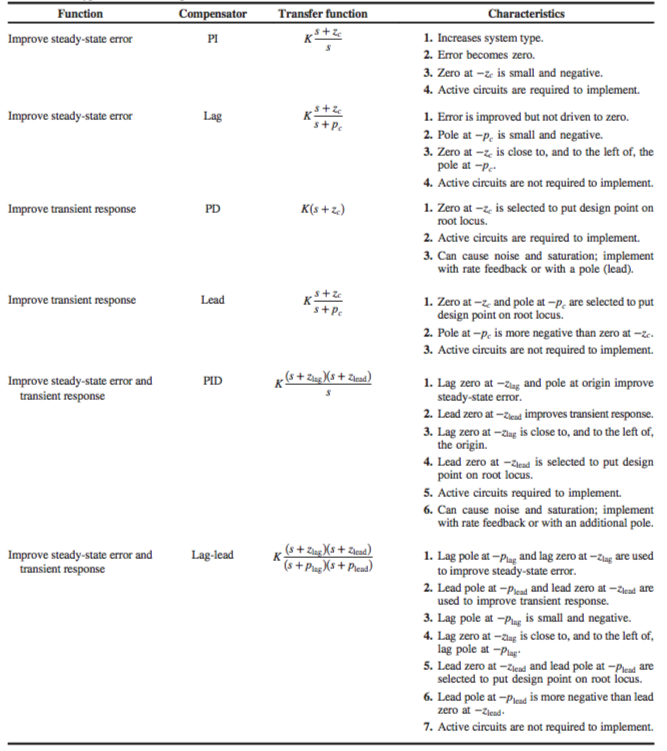
\includegraphics[width=375 px]{img/comps} \\
    \end{center}  

    \pagebreak

    %%%%%%%%%%%%%%%%%%%%%%%%%%%%%%%%%%%%%%%%%%%%%%%%%%%

    \section{Frequency Response Techniques}

    \pagebreak

    %%%%%%%%%%%%%%%%%%%%%%%%%%%%%%%%%%%%%%%%%%%%%%%%%%%

    \end{document}